\documentclass[USenglish]{article}

\usepackage{ifikompendiumforside}
\usepackage{graphicx}
\usepackage[acronym]{glossaries}
\usepackage[backend=biber,sorting=none]{biblatex}

\usepackage{tabularx}
\usepackage{cleveref}

\makeglossaries

% Acronyms
\newacronym{dil}{DIL}{Disconnected, Intermittent and Limited environments}

\title{Improving the performance of Web Services in Disconnected, Intermittent and Limited Environments}
\author{Joakim Johanson Lindquister}
\bibliography{references}

\begin{document}
\ififorside{}

\begin{abstract}
In this thesis I investigate different techniques to improve the performance of Web services in typical tactical network environments.
\end{abstract}
\pagebreak

\tableofcontents
\listoftables
\listoffigures

\pagebreak


\part{Introduction}
% Nato mange land -> mange forskjellige systemer -> viktig med standarer -> SOA og Web Services
% Så diskuter tactical networks
% Så presenter problemet - > så en oversikt over hva jeg skal gjøre med problemet
Military units may operate under conditions where the reliability of the network connection is low. They operate far from existing communication infrastructure and rely only on wireless communication. Such networks are often characterized by unreliable connections with low bandwidth and high error rates making communication difficult. In a military scenario it is necessary for units at all operational levels to seamlessly exchange information across different types of communication systems. In NATO, this concept is referred to as Network Enabled Capability(NEC). Furthermore, in a feasibility study, NATO identified the Service Oriented Architecture and Web Services as key enablers\cite{nnec-study}.

Web services is well tested in civil environments where the network is stable and the bandwidth is abundant. In contrast military tactical networks may suffer from high error rates and low bandwidth.

Different optimization techniques can be applied to reduce application overhead aswell as using specialized transport protocols, can overcome the challenges of mentioned networks.
%Få det bedre
Expensive to alter and build own properary solutions, better to use commercial off-the-shelf software. Therefore, by putting the optimization in proxies, the client and services can remain unchange while the proxy handles the optimalization.

In this thesis I investigate optimalization techniques implemented in a proxy pair.

\section{Background and Motivation}

\subsection{Web services}
NATO has chosen Web services as the technology for achieving interoperability with respect to machine-to-machine information exchange in NATO. The World Wide Web Consortium has defined Web Services as\cite{wrc-web-service}:
\paragraph{}
\textit{A Web service is a software system designed to support interoperable machine-to-machine interaction over a network. It has an interface described in a machine-processable format (specifically WSDL). Other systems interact with the Web service in a manner prescribed by its description using SOAP-messages, typically conveyed using HTTP with an XML serialization in conjunction with other Web-related standards.}
\paragraph{}
However, there also exist other types of Web services which does not follow this definition. RESTful web services let users manipulate data using a set of stateless operations. REST services have gained a lot of traction in the civil industry in the latest years.

% Trekk inn Service Oriented Architecture. Pek på at NATO har valgt dette som standard.

\subsection{Tactical networks}
Mobile tactical networks are characterized by that the units use tactical
communication equipment which includes technologies like VHF, UHF, HF, tactical
broadband and satellites. Examples of such units are mobile units like vehicles,
foot soldiers and field headquarters. These types of networks have low
bandwidth, possibly high delay, high error rates and frequent disconnections.
They are often called disadvantaged grids or DIL. NATO studies has
identified such networks to have the following characteristics:

\paragraph{}
\textit{Disadvantaged grids are characterized by low bandwidth, variable
throughput, unreliable connectivity, and energy constraints imposed by the
wireless communications grid that link the
nodes}\cite{nato-disadvantaged-grids}.

\paragraph{}
These constrains of mobile tactical networks are central in order to understand the problem at hand, and I will therefore explain the concepts here:

\begin{description}
\item[Bandwidth and throughput] The terms bandwidth and throughput are used interchangeably in the networking community and refers to the data transfer rate; how fast data can be transported from one point to another in given time period. This is often expressed in bits per second.
\item[Unreliable connectivity] Units that are participating in a tactical network are highly mobile and may disconnect from a network either voluntarily or not. Unplanned loss of connectivity can be due to various reasons, such as loss of signal or equipment malfunction.
\item[Energy constraints imposed by the wireless communication grid] The battery capacity and the transmission range of the communication equipment for mobile units may be limited. Another issue is that in some cases military units are required to enter radio silence in order to avoid being detected by the enemy. During radio silence units may only receive data and not send any.
\end{description}

Theese constrains imposes some challenges when employing Web services in tactical networks. In paper X, tree areas that need to be addresses are identified\cite{IST-118}.

\subsubsection{End-to-end connections}
\subsubsection{Network heterogeneity}
\subsubsection{Web Service overhead}

\section{Problem Statement}
Most of the Web Service solutions used today are aimed for civilian use and does
not necessarily perform well in military environments. In contrast to civilian
networks where bandwidth are abundant, mobile tactical networks may suffer
from high error rates and low bandwidth.

In my master thesis I will investigate different optimization techniques that
can be applied to improve communication. In order for the clients and services
 to remain interoperable the optimization techniques will be placed in proxies.

The Web Services will communicate with his counter part over HTTP as regular,
with all traffic going umerkelig through the proxy. The Web Service itself does
not need to pay attention to the bad connectivity, the proxy will choose the
appropriate protocol and configuration.

\section{Premises}
Ikke endre web-servicene.

\section{Scope and Limitations}
Snevre inn oppgaven.

\section{Research Methodology}

\section{Contribution}
The outcome of this thesis is an reccomandation regarding which optimizations techniques which can be used in DIL to enhance the performance of Web services.

\section{Outline}
Hvordan er resten av oppgaven strukturert.


%%%%% BACKGROUND %%%%
\part{Background}
In this part, I will present relevant technologies.
\section{Related Work}
Diskuterer eksisterende arbeid.
\section{DIL}
\gls{dil} definer hva DIL er og hvilke begrensninger det legger.

\section{Optimization techniques}
Web services enabels interoperability betweens system, but also increase the information overhead, requriering higher data rate demands. By using proxies, we can freely choose the communcations protocols and configurations between the proxy pair without altering the Web Services themself. In this thesis I will investigate different techniques in order to optimize the communcation between a Web Service and a Web Service client. \Cref{table:optimalization-overview} lists an overview of possible optimalization techniques studied in this thesis.
\\ \\ \\

%%%%%%%% TABLE OPTIMALIZATION OVERVIEW %%%%%%%%%%%%%
\begin{table}[h]
\begin{tabularx}{\textwidth}{| X | X |}
\hline
  \textbf{Protocol Stack} & \textbf{Optimalization possibilities} \\ \hline
  The application & Optimize the application\\ \hline
  Web service messaging: SOAP & Optimize SOAP, e.g XML compression \\ \hline
  HTTP/TCP, UDP or other transport protocols & SOAP is transport agnostic. Other protocols can be used. \\ \hline
  IP & NATO NEC feasibility study suggests that all protocols should be over IP. \\ \hline
  Lower layers & Not in the scope of this thesis. \\ \hline
\end{tabularx}
\caption{Optimalization possibillities.} \label{table:optimalization-overview}
\end{table}

\subsection{Compressing the payload}
Compress the payload using GZIP and forward it to the other proxy.

\subsection{Reducing overhead of SOAP}
HTTP/TCP is the most used transport protocol for SOAP messages, but since SOAP is transport protocol agnoistic diffrent protocols can be used.


\section{Requirement Analysis}
Diskutere CPU-bruk vs compression.
\\ \\ \\
\begin{table}[h]
\begin{tabular}{| l | l |}
\hline
  \textbf{Requirement} & \textbf{Priority} \\ \hline
  Receive and forward HTTP 1.X requests & 1\\ \hline
  Allow modifications on the payload & 1 \\ \hline
  Allow configuration of HTTP timeouts & 1 \\ \hline
  asd & 1 \\ \hline
  Support protocol X and y & 2 \\ \hline
\end{tabular}
\caption{Proxy requirements}
\end{table}

\section{Summary}



%%%% Design and implementation %%%%
\part{Design and Implementation}
\section{Overall Design}
\section{Proxy}
\subsection{Squid}
Squid is a fully-featured HTTP/1.0 proxy.
\begin{figure}[h]
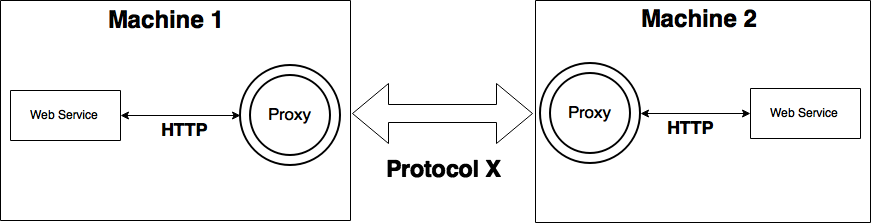
\includegraphics[scale=0.4]{images/architecture.png}
\caption{Architectural overview of proposed design}
\end{figure}



\subsection{Tuning application server configuration}

\subsection{Alternative transport protocols}

\section{Summary}

\part{Testing and Evaluation}
\section{Evaluation Tools}

\part{Conclusion and Future Work}
\section{Conclusion}

\section{Future Work}

\pagebreak
\printbibliography{}
\printglossary

\end{document}
